% Примеры правильного форматирования по ГОСТу 7.32-2017

% Пример вставки рисунка по ГОСТу
\begin{figure}[H]
\centering
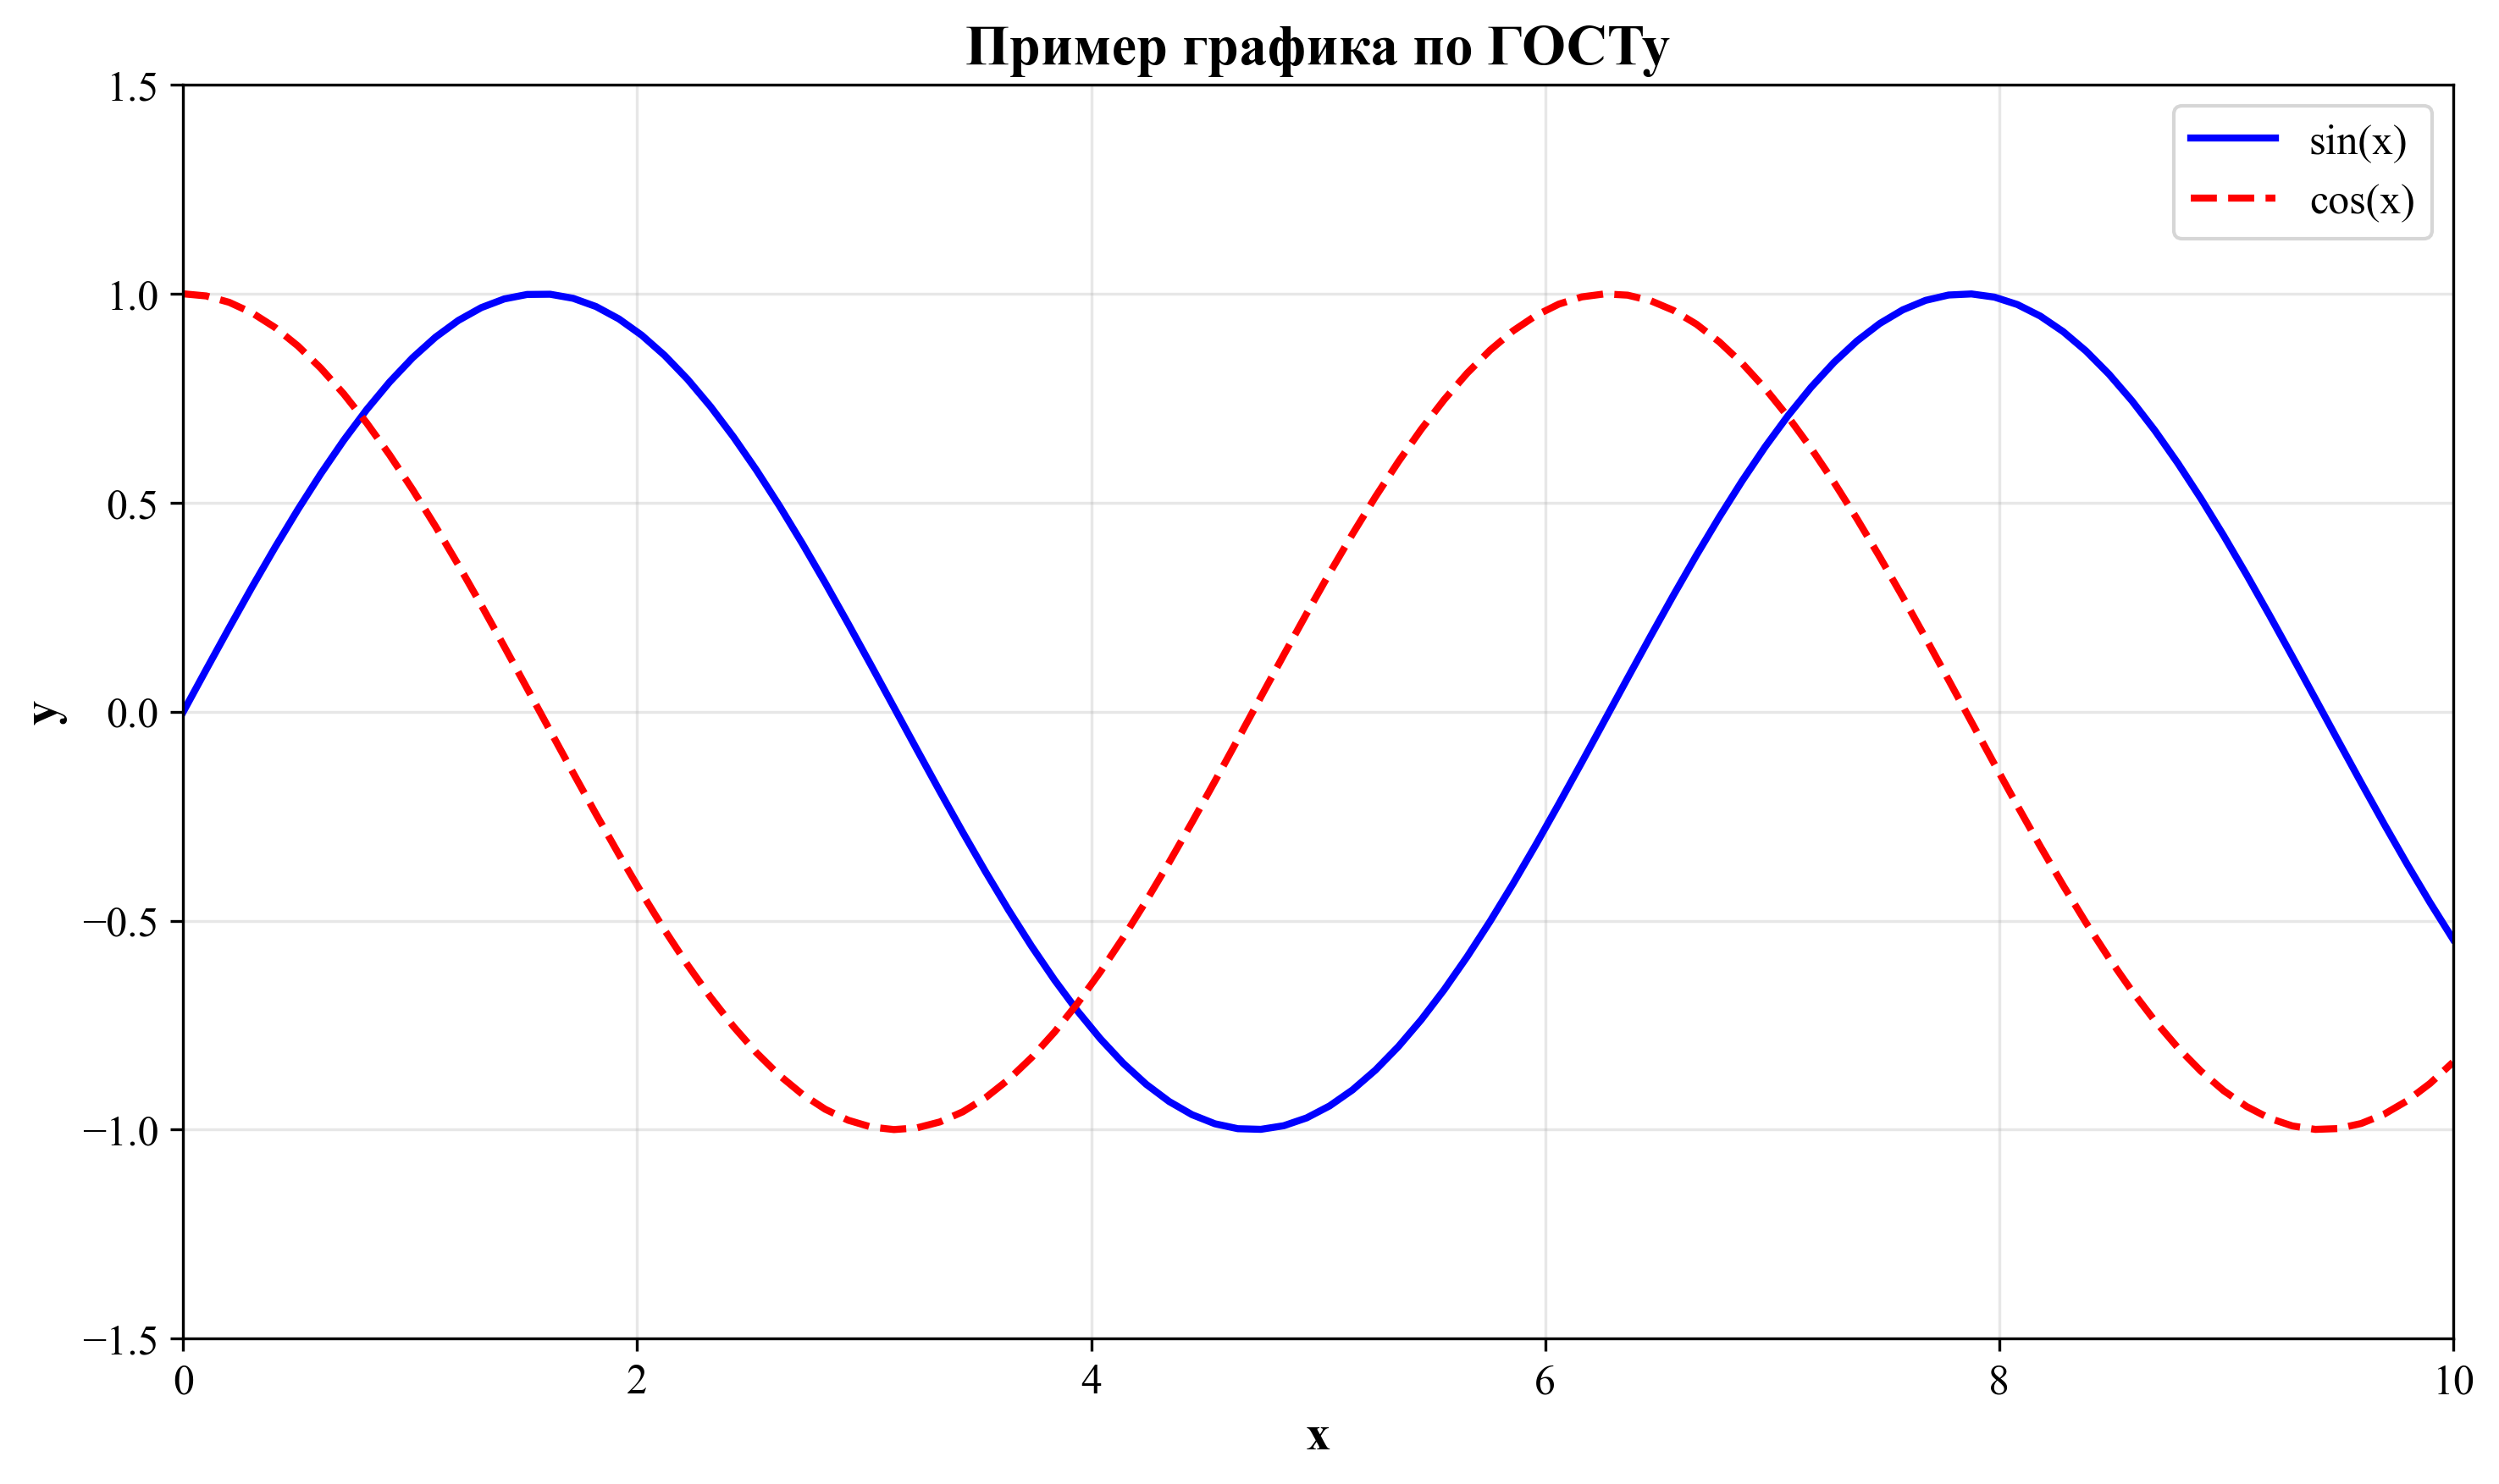
\includegraphics[width=0.6\textwidth]{images/example_plot.png}
\caption{Название рисунка (подпись должна быть краткой и точной)}
\label{fig:example}
\end{figure}

% Пример ссылки на рисунок
Согласно рисунку~\ref{fig:example}, видно что...

% Пример таблицы по ГОСТу
\begin{table}[H]
\centering
\caption{Название таблицы}
\begin{tabular}{|l|c|r|}
\hline
\multicolumn{3}{|c|}{\textbf{Заголовок таблицы}} \\
\hline
Столбец 1 & Столбец 2 & Столбец 3 \\
\hline
Данные 1 & Данные 2 & Данные 3 \\
Данные 4 & Данные 5 & Данные 6 \\
\hline
\end{tabular}
\label{tab:example}
\end{table}

% Пример ссылки на таблицу
В таблице~\ref{tab:example} представлены...

% Пример формулы по ГОСТу
\begin{equation}
E = mc^2
\label{eq:einstein}
\end{equation}

% Пример ссылки на формулу
Согласно формуле~\ref{eq:einstein}...

% Пример списка по ГОСТу
\begin{enumerate}
    \item Первый пункт;
    \item Второй пункт;
    \item Третий пункт.
\end{enumerate}

% Пример подсписка
\begin{enumerate}
    \item Первый пункт:
    \begin{enumerate}
        \item подпункт 1;
        \item подпункт 2;
    \end{enumerate}
    \item Второй пункт.
\end{enumerate}

% Пример цитирования по ГОСТу
Согласно исследованиям~\cite{example_book}, можно сделать вывод...

% Пример примечания
\begin{quote}
\textbf{Примечание} --- Текст примечания.
\end{quote}
